\documentclass[letterpaper, 10 pt, conference]{ieeeconf}
\usepackage{graphicx}
\usepackage{float}
\usepackage{listings}
\IEEEoverridecommandlockouts                             \overrideIEEEmargins
\title{\LARGE \bf
Custom Bootloaded Raspberry Pi Zero (without SD card)
}%
\author{Alok Ranjan Kesari$^{1}$, Tarun Chandrakar$^{2}$, and Dr. G. V. V. Sharma$^{3}$% 
\thanks{$^{1}$Alok Ranjan Kesari is a Research Engineer with the Department of Electrical Engineering, IIT Hyderabad
        {\tt\small arkesari@iith.ac.in}}%
\thanks{$^{2}$Tarun Chandrakar is a Project Coordinator with the Department of Electrical Engineering, IIT Hyderabad
        {\tt\small tarunchandrakar@iith.ac.in}}%
\thanks{$^{3}$ G. V. V. Sharma is with the Department of Electrical Engineering, IIT Hyderabad
        {\tt\small gadepall@iith.ac.in}}%
}

\begin{document}

\maketitle
\thispagestyle{empty}
\pagestyle{empty}
\tableofcontents

%%%%%%%%%%%%%%%%%%%%%%%%%%%%%%%%%%%%%%%%%%%%%%%%%%%%%%%%

\section{Components}
\begin{table}[htbp]
\centering
\resizebox{0.65\columnwidth}{!}{%
\begin{tabular}{|l|c|}
\hline
\textbf{Components} & \textbf{Quantity} \\ \hline
RaspberryPi Zero    & 1                 \\ \hline
Raspberry Pi3  & 1                 \\ \hline
LED                 & 1                 \\ \hline
Resistor            & 1                 \\ \hline
Jumper Wires (M to F)        & 5                  \\ \hline
\end{tabular}%
}
\label{components}
\end{table}

\section{Hardware Setup}

\begin{figure}[thpb]
\centering
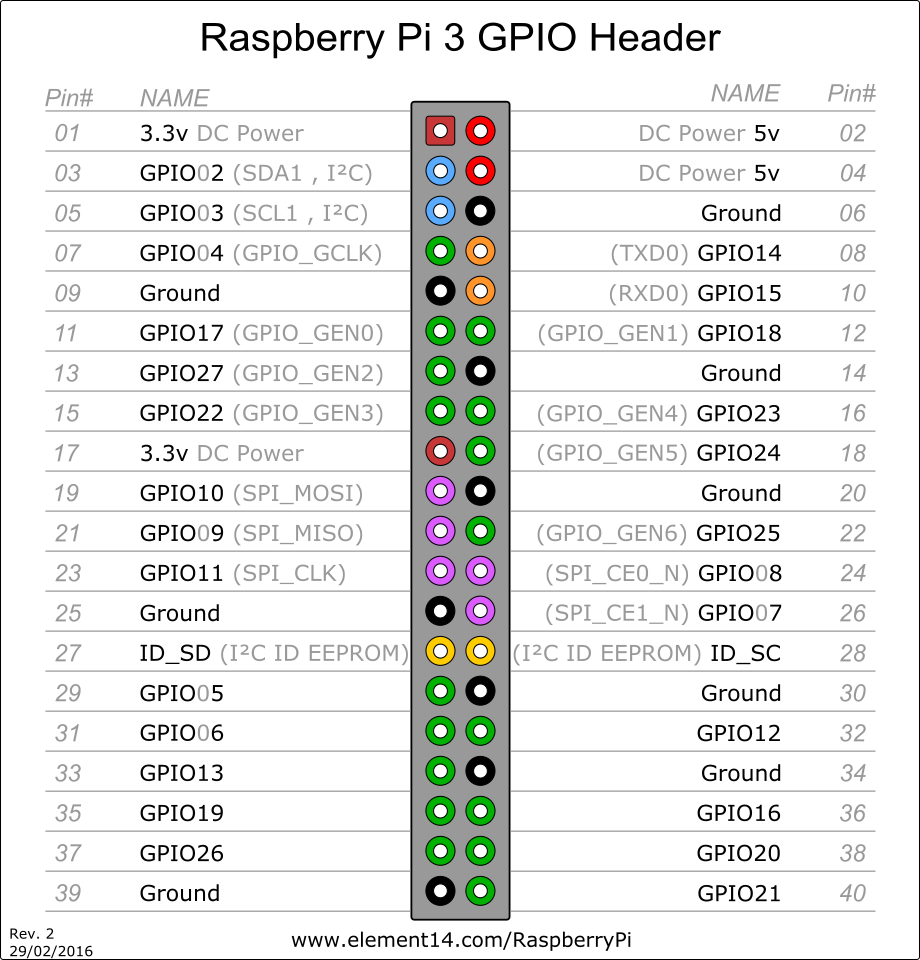
\includegraphics[width=\columnwidth]{./figs/rasp.eps}
\caption{Raspberry Pi Pin Configuration}
\label{rasp}
\end{figure}


\begin{table}[htbp]
\centering
\resizebox{0.5\columnwidth}{!}{%
\begin{tabular}{|c|c|}
\hline
\textbf{STM32 Pins} & \textbf{LED}       \\ \hline
GPIO20               & +ve                \\ \hline
GND                 & -ve (via resistor) \\ \hline
\end{tabular}%
}
\caption{RPi0and LED connection}
\label{stm32}
\end{table}

\begin{figure}[thpb]
\centering
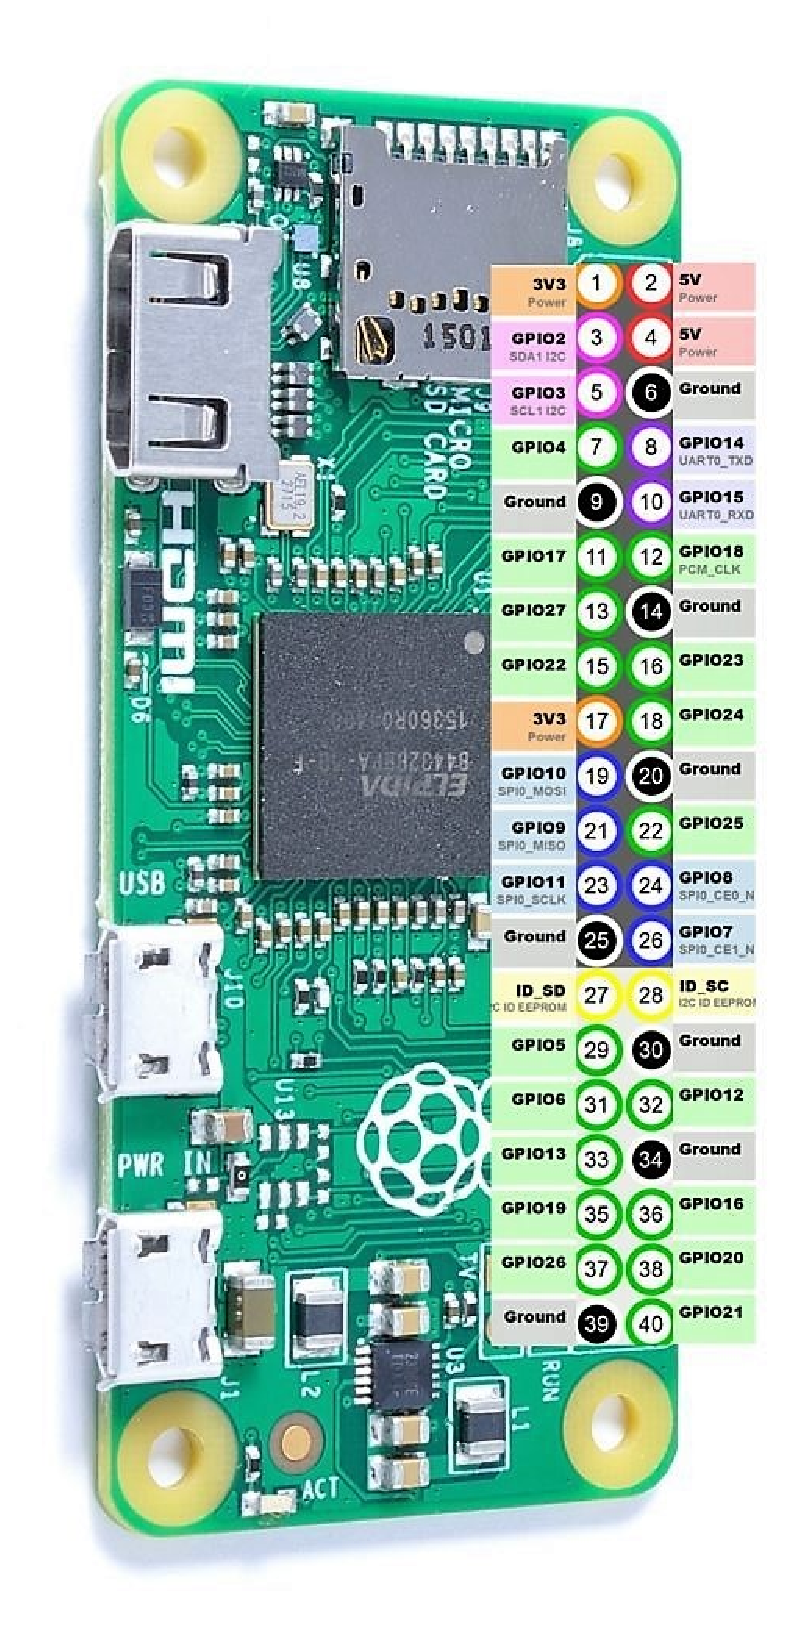
\includegraphics[width=\columnwidth]{./figs/pizero.eps}
\caption{Pi Zero Pin Configuration}
\label{stm32}
\end{figure}

\section{Software Setup}
\subsection{Installation and Configuration}
\begin{lstlisting}[frame=single, breaklines]
cd ~
git clone https://github.com/gadepall/PiZero
sudo chmod +x -R PiZero
cd PiZero

./run.sh
\end{lstlisting}
\end{document}
